% !TeX program = pdflatex
% Part III of the godsil-gutman-lean series.
% Walks that Forget the Cycles — a machine-checked bijection between tree-like walks
% of a graph and walks on Godsil's path tree, in Lean 4.
% Build: pdflatex path-tree-walks-lean.tex  (twice, for refs)

\documentclass[11pt]{article}
\usepackage[T1]{fontenc}
\usepackage{lmodern}
\usepackage{amsmath,amssymb,amsthm,booktabs,graphicx,hyperref}
\usepackage{xurl}
\usepackage[table]{xcolor}
\definecolor{ggteal}{HTML}{1B6F8C}
\definecolor{ggband}{HTML}{DCE7EB}
\definecolor{ggamber}{HTML}{E08A1E}
\usepackage[margin=1in]{geometry}
\usepackage{microtype}
\usepackage[most]{tcolorbox}
\usepackage{tikz}
\usetikzlibrary{arrows.meta,positioning}
\setlength{\emergencystretch}{2em}
\newtheorem{theorem}{Theorem}
\newtheorem{lemma}{Lemma}
\newtheorem{definition}{Definition}
\newcommand{\lean}[1]{\texttt{#1}}
\newcommand{\Z}{\mathbb{Z}}
\newcommand{\R}{\mathbb{R}}
\newcommand{\N}{\mathbb{N}}
\DeclareMathOperator{\tr}{tr}
\hypersetup{colorlinks=true,linkcolor=ggteal,citecolor=ggteal,urlcolor=ggteal}
\newtcbox{\keybox}{on line,boxrule=0.9pt,colframe=ggteal,colback=ggband!40,
  arc=3pt,left=8pt,right=8pt,top=5pt,bottom=5pt}
\newcommand{\keyeq}[1]{\begin{center}\keybox{$\displaystyle #1$}\end{center}}

\title{\bf Walks that Forget the Cycles\\[4pt]
  \large\normalfont A machine-checked bijection between tree-like walks of a graph
  and walks on Godsil's path tree, in Lean~4}
\author{Carles Mar\'in\thanks{Formalized with AI assistance (Claude, Anthropic); the mathematics
and all claims are the author's responsibility. The methodology is discussed in
Section~\ref{sec:implications}.}\\[3pt]
  \normalsize Independent researcher\\
  \normalsize \texttt{karlesmarin@gmail.com}}
\date{June 2026}

\begin{document}
\maketitle

\begin{abstract}
This is the third piece of a series that builds, in Lean~4 / Mathlib, the two sides of the
matching/Ihara trace formula. In \emph{Unfolding a Graph into a Tree}~\cite{PartII} I used Godsil's
\emph{path tree} $T(G,v)$ to prove that the matching polynomial of a graph is real-rooted: the path
tree is a forest, and a forest carries a symmetric spectrum. Here I put the \emph{same forest} to a
second use. A closed walk of $G$ is \emph{tree-like} when it never knowingly closes a cycle---at
every step it either advances to a fresh vertex or backtracks to its parent, exactly as if it were
walking on a tree. I give a machine-checked, \lean{sorry}-free proof that the tree-like closed walks
of $G$ based at $v$ are in length-preserving bijection with the closed walks of $T(G,v)$ based at its
root, realized by the down-projection $\pi\colon T(G,v)\to G$ that sends a path to its endpoint. As a
corollary the tree-like walk count becomes a sum of adjacency-matrix powers of the path trees,
\[
  \mathrm{treeLikeWalkCount}(G,k)\;=\;\sum_{v}\bigl[A(T(G,v))^{k}\bigr]_{\mathrm{root},\mathrm{root}},
\]
and, since each $T(G,v)$ is a forest, its matching polynomial equals the characteristic polynomial of
its adjacency matrix. I have not found a prior formalization of Godsil's path tree as a
walk-counting object, of the resulting bijection, or of the intrinsic ``tree-like'' predicate, in
any proof assistant. I am exact about the boundary: this paper builds the \emph{combinatorial} half
of Godsil's moment theorem $p_k=\sum_i\theta_i^{k}=\mathrm{treeLikeWalkCount}(G,k)$. The remaining
\emph{spectral} half---the single-entry resolvent identity and the univariate Newton step that turn
$[A(T)^k]_{\mathrm{root}}$ into a coefficient of $\mu(G-v)/\mu(G)$---is mapped in
Section~\ref{sec:boundary}, not built. None of this is new mathematics; the contribution is the
formalization, and the fact that the path tree now counts walks in the same library where it already
diagonalizes a spectrum.
\end{abstract}

\noindent\emph{Reader's map.} If you read only one thing, read
Theorem~\ref{thm:bij}---the bijection---and the one-line reason it holds: the path tree is the graph
\emph{unrolled} until paths self-intersect, an \emph{immersion} of $G$ in which a walk lifts at most
one way, and lifts at all exactly when it is tree-like. Everything else is the careful version of
that sentence: a local-injectivity lemma (Section~\ref{sec:inj}), a \lean{liftSeq}$\leftrightarrow$path
invariant that makes ``tree-like'' computable and matches it to the lift (Section~\ref{sec:inv}), and
the lift itself (Section~\ref{sec:surj}). The honest limit---the spectral half is mapped, not
built---is stated as plainly as the result.

\begin{figure}[h]
\centering
\resizebox{\textwidth}{!}{%
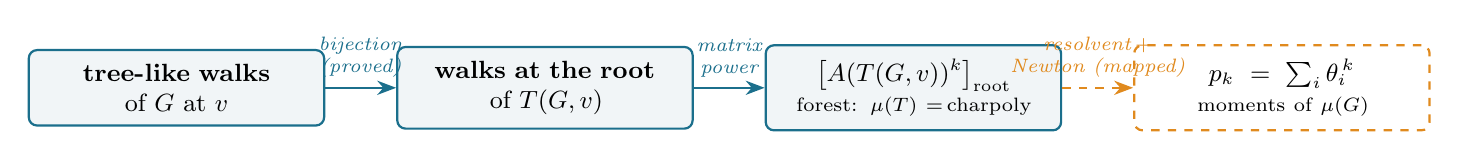
\begin{tikzpicture}[
  node distance=5mm and 9mm,
  box/.style={draw=ggteal,fill=ggband!40,rounded corners=3pt,line width=0.8pt,
    align=center,inner sep=5pt,text width=34mm,font=\small},
  mbox/.style={draw=ggamber,fill=white,rounded corners=3pt,line width=0.8pt,dashed,
    align=center,inner sep=5pt,text width=34mm,font=\small},
  arr/.style={-{Stealth[length=2.4mm]},ggteal,line width=0.9pt},
  marr/.style={-{Stealth[length=2.4mm]},ggamber,line width=0.9pt,dashed},
  lab/.style={font=\scriptsize\itshape,align=center}]
\node[box] (tl) {\textbf{tree-like walks}\\of $G$ at $v$};
\node[box,right=of tl] (pt) {\textbf{walks at the root}\\of $T(G,v)$};
\node[box,right=of pt] (am) {$\bigl[A(T(G,v))^k\bigr]_{\mathrm{root}}$\\{\scriptsize forest: $\mu(T)=$\,charpoly}};
\node[mbox,right=of am] (pk) {$p_k=\sum_i\theta_i^{\,k}$\\{\scriptsize moments of $\mu(G)$}};
\draw[arr] (tl) -- node[lab,above,text=ggteal]{bijection\\(proved)} (pt);
\draw[arr] (pt) -- node[lab,above,text=ggteal]{matrix\\power} (am);
\draw[marr] (am) -- node[lab,above,text=ggamber]{resolvent\,$+$\\Newton (mapped)} (pk);
\end{tikzpicture}}
\caption{The route of the paper, and where it stops. The tree-like walk count of $G$ equals the walk
count at the root of Godsil's path tree (the bijection, Theorem~\ref{thm:bij}), which is a power of the
tree's adjacency matrix (Theorem~\ref{thm:spectral}); and each path tree is a forest, so that matrix's
characteristic polynomial is the matching polynomial (Theorem~\ref{thm:forest}). The solid arrows are
machine-checked here; the dashed arrow to the moments $p_k$---the single-entry resolvent, Godsil's
ratio identity, and the univariate Newton step---is mapped in Section~\ref{sec:boundary}, not built.}
\label{fig:spine}
\end{figure}

% ---------------------------------------------------------------
\section{Introduction: one tree, two harvests}
\label{sec:intro}

\emph{When does a walk on a graph fail to notice that the graph has cycles---and why should counting
those forgetful walks recover the moments of a polynomial that is the characteristic polynomial of no
matrix at all?} The two halves of that question turn out to have a single answer, a tree; this paper
machine-checks the combinatorial half of it.

Answering it---and explaining why a single combinatorial device settles two facts about a graph that
look unrelated---asks three threads of history to meet.

\paragraph{A polynomial with real roots and no matrix (1972).} A finite graph $G$ has a matching
polynomial $\mu(G,x)=\sum_{k}(-1)^k m_k(G)\,x^{n-2k}$, where $m_k(G)$ counts its $k$-edge
matchings~\cite{Farrell1979,LovaszPlummer}. In 1972 Heilmann and Lieb, studying monomer--dimer
systems in statistical mechanics, proved that its roots are always real~\cite{HeilmannLieb}---a
phase-transition statement in physics, a spectral one in combinatorics. But real roots are the
signature of a \emph{symmetric matrix}, and $\mu(G)$ is the characteristic polynomial of no fixed
matrix unless $G$ is a forest. So the question sharpens: if there is no matrix, where do the real
roots, and the combinatorial content of their power sums $p_k=\sum_i\theta_i^{k}$, come from?

\paragraph{One tree, two theorems (1981).} Godsil's answer was a single device~\cite{Godsil1981a,
Godsil1981b,GodsilBook}. Given a vertex $v$, the \emph{path tree} $T(G,v)$ has as vertices the simple
paths of $G$ that start at $v$, with one path joined to another when the second extends the first by a
single edge. It is a forest---the finite truncation of the \emph{universal cover} of $G$ unrolled from
$v$---and from it Godsil drew two conclusions. First, $\mu(G)\mid\mu(T(G,v))$, and a forest's matching
polynomial \emph{is} the characteristic polynomial of its adjacency matrix, hence real-rooted; this
recovers Heilmann--Lieb, and is what Part~II of this series~\cite{PartII} formalized. Second---the
subject of this paper---the path tree \emph{counts walks}.

\paragraph{Walks, covers, and a trace formula.} The universal cover is the deeper object behind the
finite tree: the spectral radius of the infinite $(\Delta-1)$-regular tree is $2\sqrt{\Delta-1}$, the
\emph{Ramanujan} edge, which is also Godsil's bound on the matching roots, and the cover's spectrum is
governed by the matching polynomial~\cite{AngelFriedmanHoory,Spier2025}. On the finite side this is a
\emph{trace formula}: $\tr(A^k)$ counts \emph{all} closed walks of $G$, while $p_k$ counts only the
\emph{tree-like} ones; below the girth every walk is tree-like, so the two agree, and the first gap
counts shortest cycles. The cycle side, $\tr(A^k)$ and its non-backtracking refinement, is the
\emph{Bass} companion of this series~\cite{Bass,Hashimoto,IharaBass}; this paper builds the
combinatorial half of the tree side.

A closed walk of $G$ is \emph{tree-like} when, viewed step by step, it only ever extends to a new
vertex or retreats to the vertex it came from: it never traverses an edge back to an earlier,
non-parent vertex, so it never knowingly encloses a cycle. (It may still, in aggregate, traverse the
three edges of a triangle---as long as each intermediate \emph{path} stays simple; this is exactly
where the naive definition fails, Figure~\ref{fig:moments}.) Godsil's observation is that these are
precisely the walks $G$ inherits from $T(G,v)$: a closed walk at the root of the path tree, pushed
down to $G$ by recording only the current endpoint, is a tree-like closed walk at $v$, and every
tree-like walk arises this way, uniquely (Figure~\ref{fig:bij}). Summing over $v$ and over the
length-$k$ walks gives $\mathrm{treeLikeWalkCount}(G,k)$, and the moment theorem identifies it with
$p_k(G)$.

\paragraph{Why formalize it.} The matching polynomial sits at the intersection of three of this
series' threads---real-rootedness (Parts~I--II~\cite{PartI,PartII}), the matching/Ihara trace formula
(the \emph{Bass} companion~\cite{Bass}), and, through the band edge $2\sqrt{\Delta-1}$, Ramanujan
graphs~\cite{MSS}. The trace formula has a \emph{cycle} side, $\tr(A^k)$ counting all closed walks,
and a \emph{tree} side, $p_k$ counting tree-like ones; below the girth they coincide, and the first
gap is a count of shortest cycles. To state that bridge inside a proof assistant one needs the
tree side as an honest object, and the tree side is precisely a statement about the path tree.
Part~II built the path tree for its spectrum; this paper teaches the same Lean object to count.

\paragraph{What is new here, and what is not.} The mathematics is Godsil's. The contribution is the
machine-checked construction: the path tree as a walk-counting graph, the down-projection as a graph
homomorphism that is an \emph{immersion}, an intrinsic decidable predicate \lean{IsTreeLike} computing
the lift as a stack discipline, the invariant tying that stack to the current path-tree vertex, the
lift in the surjective direction, and the resulting cardinality bijection. For none of these could I
find a prior formalization in any proof assistant. The headline depends only on the three standard
axioms (\lean{propext}, \lean{Classical.choice}, \lean{Quot.sound}); there is no \lean{sorry}.

% ---------------------------------------------------------------
\section{The two sides, kept apart}
\label{sec:objects}

\emph{What, exactly, are we matching---and how do we keep the two sides from being the same object
wearing two hats?} A bijection only says something when its ends are defined without reference to each
other; so I fix both, and only later let them meet. Throughout, $G$ is a \lean{SimpleGraph} on a
vertex type $V$, and $v\in V$ is a base point. I reuse the path tree of Part~II verbatim.

\begin{definition}[Path tree, \lean{pathTree}]
The vertices of $T(G,v)=\lean{pathTree}\,G\,v$ are the simple paths of $G$ starting at $v$
(\lean{PathFrom}\,$v=\Sigma_{u}\,G.\mathrm{Path}\,v\,u$). Two are adjacent when one is obtained from
the other by appending a single edge at its end (\lean{Grows}). The root is the trivial path at $v$
(\lean{pathTreeRoot}). It is a forest: \lean{pathTree\_isAcyclic}.
\end{definition}

\begin{definition}[Down-projection, \lean{pathTreeProj}]
$\pi\colon T(G,v)\to G$ sends a path to its endpoint, $\pi\langle u,p\rangle=u$. Adjacency in the
path tree means one path extends the other by an edge, so the two endpoints are adjacent in $G$;
hence $\pi$ is a graph homomorphism, and $\pi(\mathrm{root})=v$.
\end{definition}

The tree-like predicate is defined intrinsically, without reference to the path tree, so that the
two sides of the bijection are genuinely different objects to be matched. A closed walk
$w$ at $v$ is fed, vertex by vertex (its support past the first entry), to a deterministic
\emph{lift} \lean{liftSeq} that threads a stack---the current simple path from $v$. For each next
vertex $c$: if $c$ is not on the stack, \emph{push} it (an \textsc{extend}); if $c$ is the
penultimate vertex of the stack, \emph{pop} (a \textsc{retreat} to the parent); otherwise the lift
\emph{fails}. The two cases are mutually exclusive, so the lift is a fold.

\begin{definition}[Tree-like, \lean{Walk.IsTreeLike}]
$w$ is \emph{tree-like} iff its lift, started from the root stack $[v]$, returns to $[v]$:
$\lean{liftSeq}\;w.\mathrm{support}.\mathrm{tail}\;[v]=\lean{some}\,[v]$. This is decidable.
\end{definition}

This definition is the corrected one. The naive choice---``the edge-support of $w$ is acyclic''---is
\emph{wrong} for the moment theorem: on $K_4$ with $k=6$ it undercounts ($276$ against $p_6=324$),
because a tree-like walk may traverse a cycle's edges in aggregate. The \lean{liftSeq} predicate was
validated numerically against the matching power sums on $P_4,C_4,C_5,K_4$ and the Petersen and
$K_{3,3}$ graphs for $k\le8$ before it was formalized (Figure~\ref{fig:moments}).

\begin{figure}[t]
  \centering
  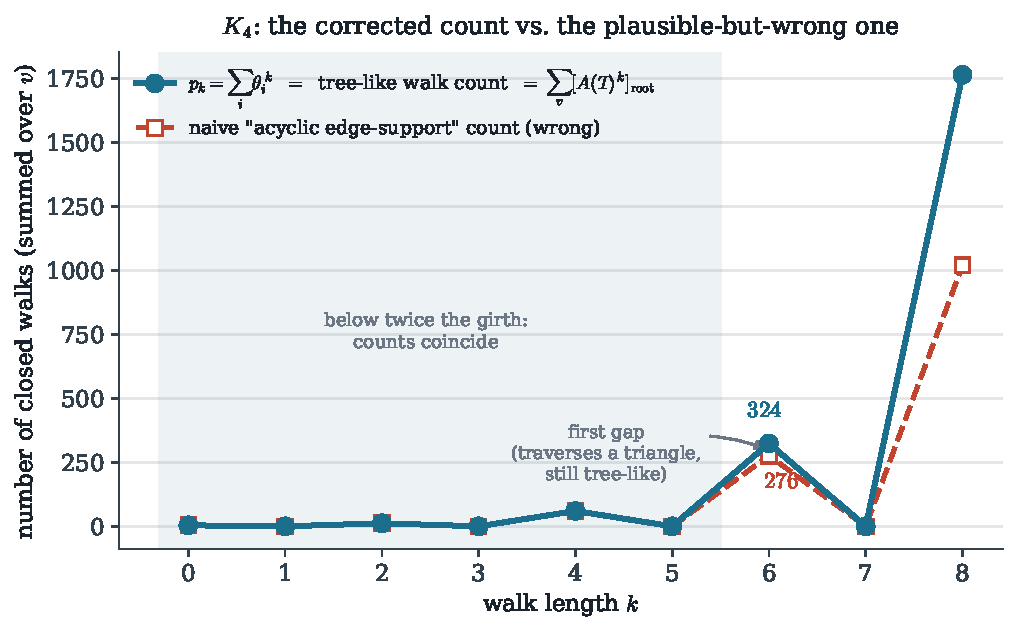
\includegraphics[width=0.82\textwidth]{figures/pt_fig2_moments.pdf}
  \caption{Why the definition matters, on $K_4$. The matching power sums $p_k$ (teal) coincide with
  the tree-like / path-tree count for every $k$---this paper's bijection makes the second equality
  exact. The plausible ``acyclic edge-support'' count (red) agrees through $k=5$ but then undercounts,
  $276$ against $324$ at $k=6$, because a tree-like walk may traverse all three edges of a triangle
  while every intermediate path stays simple. A cheap numerical check caught the wrong definition
  before any formal effort was spent on it.}
  \label{fig:moments}
\end{figure}

% ---------------------------------------------------------------
\section{The result}
\label{sec:result}

\begin{theorem}[The bijection, \lean{card\_treeLike\_eq\_pathTreeWalks}]\label{thm:bij}
For every finite graph $G$, base point $v$, and length $k$, the map $W\mapsto W.\mathrm{map}\,\pi$ is
a bijection from the closed walks of length $k$ at the root of $T(G,v)$ onto the tree-like closed
walks of length $k$ of $G$ at $v$. In particular their cardinalities agree:
\keyeq{\#\{\,\text{tree-like walks of }G\text{ at }v,\ \text{length }k\,\}
   \;=\;\#\{\,\text{walks at the root of }T(G,v),\ \text{length }k\,\}.}
\end{theorem}

\begin{figure}[t]
  \centering
  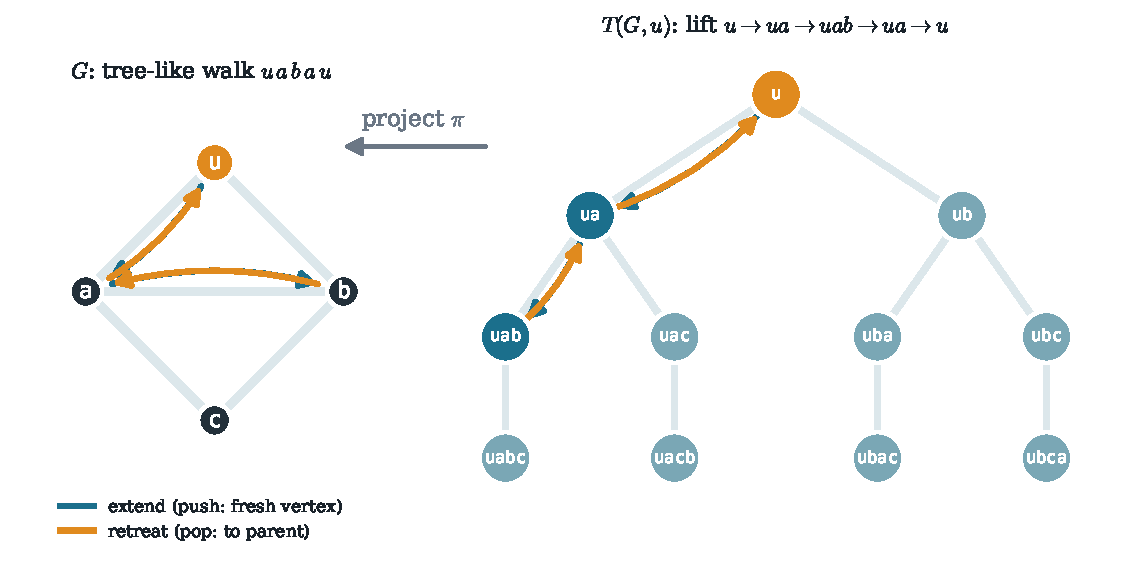
\includegraphics[width=0.96\textwidth]{figures/pt_fig1_bijection.pdf}
  \caption{The bijection on the diamond $G=K_4-e$, root $u$. A closed walk at the root of the path
  tree $T(G,u)$ (right), $u\to ua\to uab\to ua\to u$, projects under $\pi$ (a path $\mapsto$ its
  endpoint) to a tree-like closed walk of $G$ (left), $u\,a\,b\,a\,u$. Each step is an \textsc{extend}
  (teal, advance to a fresh vertex / push) or a \textsc{retreat} (amber, backtrack to the parent /
  pop). The walk on the left traverses the edges $ua,ab$ outward and retraces them back; the lift on
  the right makes the path history explicit, and is the unique walk over it.}
  \label{fig:bij}
\end{figure}

\emph{What does it take to trust a bijection?} A map, and its promise kept in two directions. The
map is $\pi$ read on whole walks, $W\mapsto W.\mathrm{map}\,\pi$; its promise is three facts, and the
three proof sections that follow are, in order, exactly those three. The map must \emph{land where it
should}: a projected tree-walk is always tree-like, so $\pi$ carries the tree's walks \emph{into}
$G$'s tree-like ones (Lemma~\ref{lem:img}, earned in Section~\ref{sec:inv}). It must \emph{forget
nothing}: no two tree-walks cast the same shadow (Lemma~\ref{lem:inj}, Section~\ref{sec:inj}). And it
must \emph{miss nothing}: every tree-like walk is some walk's shadow---the lift exists
(Lemma~\ref{lem:surj}, Section~\ref{sec:surj}). Land, injective, surjective; that is the whole of
Theorem~\ref{thm:bij}, and the rest of the paper is those three words made precise.

\begin{lemma}[Image is tree-like, \lean{pathTreeProj\_map\_isTreeLike}]\label{lem:img}
The $\pi$-projection of any closed walk at the root of $T(G,v)$ is tree-like.
\end{lemma}

\begin{lemma}[Injectivity, \lean{pathTreeProj\_walk\_injective}]\label{lem:inj}
$W\mapsto W.\mathrm{map}\,\pi$ is injective on walks of $T(G,v)$.
\end{lemma}

\begin{lemma}[Surjectivity / the lift, \lean{exists\_root\_lift}]\label{lem:surj}
Every tree-like closed walk of $G$ at $v$ is $W.\mathrm{map}\,\pi$ for some closed walk $W$ at the
root of $T(G,v)$.
\end{lemma}

\emph{A bijection that only renames a finite set is bookkeeping---so what does this one buy?} Its
worth is that the two sides are different \emph{kinds} of object: on the left, a combinatorial count;
on the right, walks on a \emph{tree}. And a tree has a matrix. So the count on the right is a matrix
power, a matrix power is a spectral quantity, and the rename has quietly moved us onto the spectral
side, where the rest of the moment theorem lives. Two corollaries take the step.

\begin{theorem}[Spectral form, \lean{treeLikeWalkCount\_eq\_sum\_pathTree\_adjMatrix\_pow}]
\label{thm:spectral}
\[
  \mathrm{treeLikeWalkCount}(G,k)\;=\;\sum_{v\in V}\bigl[A(T(G,v))^{k}\bigr]_{\mathrm{root},\mathrm{root}}.
\]
\end{theorem}

\begin{theorem}[Forest bridge, \lean{matchingPoly\_pathTree\_eq\_charpoly}]\label{thm:forest}
Each path tree is a forest, so its matching polynomial is the characteristic polynomial of its
adjacency matrix: $\mu(T(G,v))=\mathrm{charpoly}\bigl(A(T(G,v))\bigr)$.
\end{theorem}

% ---------------------------------------------------------------
\section{The path tree is an immersion}
\label{sec:inj}

\emph{If the path tree is the graph unrolled, what stops a walk from unrolling ambiguously---from
having two different lifts?} The answer is local, and it is the whole engine of injectivity. The
neighbours of a
path-tree vertex $p$ are its unique parent (drop the last edge) and its
children (append one edge each). The projection $\pi$ sends the parent to $p$'s penultimate vertex,
which lies on $p$, and each child to its fresh endpoint, which does not; and distinct children have
distinct endpoints. So $\pi$ \emph{separates} the neighbours of every vertex:
\lean{pathTreeProj\_injOn\_neighborSet}. The parent half is Part~II's \lean{Grows.parent\_unique};
its dual \lean{Grows.child\_unique} (a one-edge extension is determined by its endpoint) is new here.

This local injectivity is exactly the immersion property: $\pi$ is locally injective but not locally
surjective---a $G$-neighbour of $p$'s endpoint that already lies on $p$ has \emph{no} preimage above
$p$. That asymmetry is the whole story. It is also an old one in a different dress: a covering map, in
the sense of Poincar\'e's topology, lifts \emph{every} path uniquely; an immersion lifts only the
paths that never double back into themselves---and ``never doubles back into a non-parent vertex'' is
precisely what tree-like means. A walk in $T(G,v)$ is determined, step by step, by its
$\pi$-image together with its start, because at each vertex the next path-tree vertex is forced by the
local injection; an induction mirroring Mathlib's \lean{Walk.map\_injective\_of\_injective}, with the
global hypothesis replaced by the local one, gives Lemma~\ref{lem:inj}.

\begin{figure}[t]
  \centering
  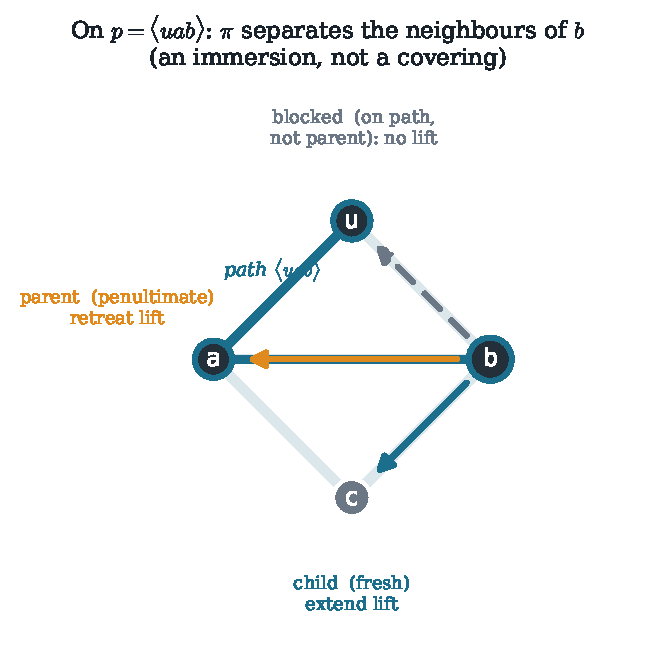
\includegraphics[width=0.62\textwidth]{figures/pt_fig4_immersion.pdf}
  \caption{The immersion, at the path-tree vertex $p=\langle uab\rangle$ (the path $u\,a\,b$, teal).
  The next step looks at the neighbours of the endpoint $b$, which in $G$ are $a$, $c$, $u$. Each falls
  into exactly one case: $a$ is the penultimate of $p$ (the \emph{parent}, a retreat), $c$ is fresh (a
  \emph{child}, an extend), and $u$ lies on $p$ but is not its parent---\emph{blocked}, with no lift
  above $p$. So $\pi$ is injective on the neighbours of $p$ but not surjective; the blocked direction
  is why the path tree is an immersion, and why a projected walk can only be tree-like.}
  \label{fig:immersion}
\end{figure}

% ---------------------------------------------------------------
\section{The \texttt{liftSeq}$\leftrightarrow$path invariant}
\label{sec:inv}

\emph{\lean{IsTreeLike} is a stack discipline on $G$ alone---the path tree appears nowhere in it---so
why should it detect exactly the walks that come from the tree?} Because the stack \emph{is} the tree
vertex in disguise. Reading a walk as a sequence of pushes and pops is the oldest move in enumerative
combinatorics---the ballot problem, von Dyck's balanced words, the Catalan numbers all live on the
same stack---and here it is the bridge, in the form of a single invariant: as one walks $T(G,v)$,
running \lean{liftSeq} on the projected walk tracks the current path-tree vertex.

\begin{lemma}[One step, \lean{liftSeq\_step}]
For a path-tree edge $s\sim y$ and any tail $M$,
$\lean{liftSeq}\,(y_1::M)\,s.\mathrm{support}=\lean{liftSeq}\,M\,y.\mathrm{support}$: a child step is a
\textsc{push}, a parent step is a \textsc{pop}.
\end{lemma}

\begin{lemma}[Invariant, \lean{liftSeq\_map\_invariant}]\label{lem:inv}
For a path-tree walk $W\colon s\to x$,
\[
  \lean{liftSeq}\,(W.\mathrm{map}\,\pi).\mathrm{support}.\mathrm{tail}\;\,s.\mathrm{support}
  =\lean{some}\,x.\mathrm{support}.
\]
\end{lemma}

Lemma~\ref{lem:img} is the case $s=x=\mathrm{root}$, whose path-support is $[v]$. The same invariant
drives the lift: it is the bookkeeping that, run in reverse, reconstructs the path-tree walk from a
tree-like walk.

\begin{figure}[t]
  \centering
  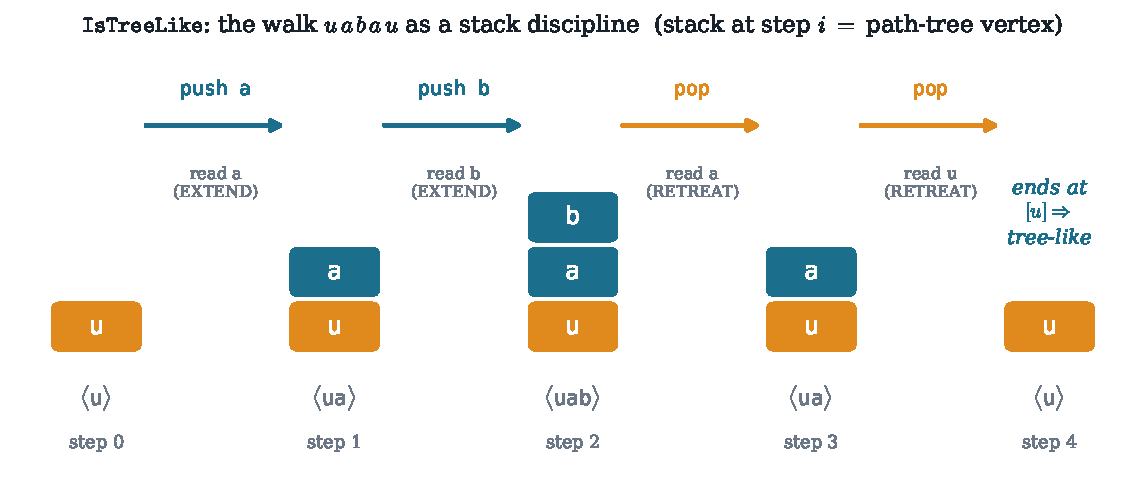
\includegraphics[width=0.97\textwidth]{figures/pt_fig3_stack.pdf}
  \caption{\lean{IsTreeLike} as a stack discipline---the \lean{liftSeq} predicate run on the walk
  $u\,a\,b\,a\,u$. The stack is the current simple path from $u$; each next vertex is read and either
  \textsc{pushed} (extend, teal: a fresh vertex) or \textsc{popped} (retreat, amber: it is the
  penultimate). The walk is tree-like iff the stack ends back at $[u]$. The stack at step $i$ is
  exactly the path-tree vertex the lift sits on---$\langle u\rangle,\langle ua\rangle,\langle uab
  \rangle,\langle ua\rangle,\langle u\rangle$---which is the content of the invariant,
  Lemma~\ref{lem:inv}.}
  \label{fig:stack}
\end{figure}

% ---------------------------------------------------------------
\section{The lift: climbing back into the tree}
\label{sec:surj}

\emph{Every tree-like walk should come from the tree---but how do we exhibit the walk it comes from,
when its very endpoints in the tree are not given but computed?} Surjectivity is the only direction
that builds a walk in the dependent type
$(T(G,v)).\mathrm{Walk}$, and its endpoints are computed, not given. The construction
(\lean{exists\_lift}) is a recursion on the $G$-walk: the hypothesis ``\lean{liftSeq} accepts $w$ from
the current vertex'' supplies, at each step, the \textsc{extend}/\textsc{retreat} decision, so there
is no failure branch. The current path-tree vertex is carried as the explicit triple
$\langle a, pp, hpp\rangle$ (endpoint, path, proof-it-is-a-path), which sidesteps the heterogeneous
equalities that a $\Sigma$-typed accumulator would force. Two further frictions are handled by the
same trick: the recursion proves equality of \emph{supports} (a \lean{List}~$V$, free of dependent
types) rather than of walks, and \lean{Walk.support\_injective} upgrades support equality to walk
equality once the endpoints are pinned down in the closed-walk corollary
(Lemma~\ref{lem:surj}). The lift returns to the root because its final path-support is $[v]$, forcing
the final tree-vertex to be the trivial path.

The bijection (Theorem~\ref{thm:bij}) is then \lean{Finset.card\_bij} on $W\mapsto W.\mathrm{map}\,\pi$,
with Lemma~\ref{lem:img} for well-definedness, Lemma~\ref{lem:inj} for injectivity, and
Lemma~\ref{lem:surj} for surjectivity; lengths are preserved because $\mathrm{map}$ preserves them.

% ---------------------------------------------------------------
\section{The boundary: what is built, and what is mapped}
\label{sec:boundary}

\emph{The bijection counts; the moment theorem equates that count with a spectrum. Where, precisely,
does the machine-checked ground end and the mapped-but-unbuilt algebra begin?} Godsil's moment theorem
is
\keyeq{p_k(G)\;=\;\sum_i\theta_i^{k}\;=\;\mathrm{treeLikeWalkCount}(G,k).}
This paper builds its \emph{combinatorial} half---everything up to and including the spectral form
(Theorem~\ref{thm:spectral}) and the forest bridge (Theorem~\ref{thm:forest}). The
\emph{spectral} half is mapped here but not formalized; I state it plainly so the reader knows
exactly where the machine-checked ground ends.

The remaining chain is standard algebra. For each path tree $T=T(G,v)$, the root--root resolvent
generates the walk counts,
\[
  \sum_{k\ge0}\bigl[A(T)^k\bigr]_{\mathrm{root}}X^{k}
  \;=\;\frac{\mathrm{charpolyRev}\bigl(A(T)_{\widehat{\mathrm{root}}}\bigr)}{\mathrm{charpolyRev}(A(T))},
\]
the single-entry case of $\mathrm{adj}(1-XA)=\det(1-XA)\,(1-XA)^{-1}$, which this library already has
in matrix form (\lean{smul\_resolventSeries\_eq\_adjugate}, \lean{coeff\_resolventSeries}). What is
\emph{not} yet in Mathlib, and is the one genuinely new linear-algebra lemma the completion needs, is
the general principal-minor identity $\mathrm{adj}(M)_{ii}=\det\bigl(M\!\restriction_{j\neq i}\bigr)$
over an arbitrary finite index type (Mathlib has only the \lean{Fin} cofactor expansion). Granting it,
the forest bridge turns each $\mathrm{charpolyRev}$ into a reversed matching polynomial; Part~II's
\lean{godsil\_identity}, $\mu(G)\,\mu(T-\mathrm{root})=\mu(G-v)\,\mu(T)$, rewrites the ratio as
$\mu(G-v)/\mu(G)$; the vertex-deletion derivative law $\sum_v\mu(G-v)=X\,\mu'(G)$ (already proved,
\lean{sum\_matchingPoly\_deleteIncidenceSet}) sums it to $\mu'(G)/\mu(G)$; and the univariate Newton
identity equates that logarithmic derivative with $\sum_k p_k X^{k}$. Matching coefficients of $X^k$
closes the theorem. The last step is itself venerable: Newton's identities, relating a polynomial's
power sums to its coefficients, were written down by Girard in 1629 and by Newton a generation later,
and Sachs' 1964 coefficient theorem reads those coefficients off the graph's own subgraphs. Two of the
links---the principal-minor lemma and the univariate-root Newton bridge---are general results absent
from Mathlib, and both are kept in the repository's \texttt{MathlibPR} staging in canonical, graph-free
form.

% ---------------------------------------------------------------
\section{Implications and methodology}
\label{sec:implications}

The author set the targets and adjudicated the mathematics; the assistant (Claude, Anthropic) drafted
the proofs and this prose. Every theorem cited here compiles \lean{sorry}-free against the pinned
Mathlib revision~\cite{Mathlib} and depends only on the three standard axioms, which the reader can
re-verify with \lean{\#print axioms}. The corrected ``tree-like'' definition is itself a small
methodological datapoint: the natural acyclic-support reading is plausible, compiles, and is
\emph{false} for the theorem it is meant to serve; a cheap numerical check against the matching power
sums caught it before any formal effort was spent, and the same check certifies the
\lean{liftSeq} definition that replaced it.

\paragraph{What it is good for---and what it is not.} The objects here are not exotic. The matching
polynomial is the monomer--dimer partition function of statistical mechanics~\cite{HeilmannLieb}; the
moments of its roots are the raw material of the method of moments for eigenvalue bounds; the bound
those moments obey, $2\sqrt{\Delta-1}$, is the threshold a graph must clear to be an expander; and the
spectral object next door, the non-backtracking operator, sets a network's percolation
threshold~\cite{Hashimoto,Bass}. This paper adds nothing to any of that. It only places one half of
the bridge those methods cross---the tree side of the trace formula---on certified ground, in the same
library as the cycle side, and leaves behind a small reusable object, the path tree, that already did
one job (a real spectrum, Part~II) and now does a second. No algorithm and no network: a foundation,
and a modest one.

The mathematics is Godsil's, four decades old. I have only carried it, carefully, into a form a
machine will check: in Part~II the path tree carries a real spectrum, and here it counts the walks a
graph mistakes for a tree. The cycle side of the matching/Ihara trace formula---$\tr(A^k)$---stands in
the same library (the \emph{Bass} companion~\cite{Bass}); should the spectral half of
Section~\ref{sec:boundary} one day be built, the tree side $p_k$ would meet it, and the trace formula
would be a single machine-checked line. That is left, without apology, for another day.

% ---------------------------------------------------------------
\section{Questions left open}
\label{sec:questions}

A formalization is also a list of the next questions, sharpened to the point where a machine could be
asked them. These are the ones this paper leaves on the table.

\begin{itemize}
\item The completion of Section~\ref{sec:boundary} hangs on one general, Mathlib-absent lemma:
the principal-minor identity $\mathrm{adj}(M)_{ii}=\det(M\!\restriction_{j\neq i})$ over an arbitrary
finite index type. Is the clean route a reindexing to \lean{Fin} and the existing cofactor expansion,
or is there a basis-free proof that never names an ordering?
\item The corrected ``tree-like'' predicate is a \emph{stack discipline}. Is it the unique reasonable
intrinsic definition, or does the free-reduction-to-trivial reading (a walk that reduces to the empty
word under backtrack cancellation) define the same class for every $k$---and if so, is the
equivalence cheaper to prove than either side of the bijection?
\item The bijection is length-preserving and vertex-local. Does it refine to an isomorphism of the
\emph{generating functions} before any spectral input, i.e. can $\sum_k(\#\text{tree-like})X^k$ be
identified with a path-tree resolvent entry purely combinatorially, leaving the matching polynomial
out until the very end?
\item Below the girth, tree-like walks are all walks, so the count equals $\tr(A^k)$ locally; the
first gap, at $k=\text{girth}$, counts shortest cycles. Can the path-tree bijection be made to
\emph{see} that gap---to produce the cycle-counting correction term as the obstruction to a walk
lifting?
\item The same forest carries the band edge $2\sqrt{\Delta-1}$ (Part~II) and, here, the walk counts
whose growth rate is that very edge. Is the Ramanujan bound on the matching roots a \emph{corollary}
of this bijection plus a comparison with the infinite $(\Delta-1)$-ary tree, formalizable without
re-entering the interlacing-families machinery?
\end{itemize}

And one to keep. \emph{When a machine certifies that a graph's tree-like walks are exactly a tree's
walks, has it proved that the graph is, for the purpose of counting, a tree---or only that we have
named the precise sense in which it refuses to be one?}

% ---------------------------------------------------------------
\begin{thebibliography}{99}

% --- the matching polynomial and its real-rootedness ---
\bibitem{HeilmannLieb} O.~J. Heilmann and E.~H. Lieb, \emph{Theory of monomer--dimer systems},
Comm.\ Math.\ Phys.\ \textbf{25} (1972), 190--232.
\bibitem{Farrell1979} E.~J. Farrell, \emph{An introduction to matching polynomials}, J.~Combin.\
Theory Ser.~B \textbf{27} (1979), 75--86.
\bibitem{LovaszPlummer} L.~Lov\'asz and M.~D. Plummer, \emph{Matching Theory}, North-Holland Math.\
Stud.\ \textbf{121}, Amsterdam, 1986.

% --- Godsil's path tree: matchings and walks ---
\bibitem{Godsil1981a} C.~D. Godsil, \emph{Matchings and walks in graphs}, J.~Graph Theory \textbf{5}
(1981), 285--297.
\bibitem{Godsil1981b} C.~D. Godsil and I.~Gutman, \emph{On the theory of the matching polynomial},
J.~Graph Theory \textbf{5} (1981), 137--144.
\bibitem{GodsilBook} C.~D. Godsil, \emph{Algebraic Combinatorics}, Chapman \& Hall, New York, 1993.

% --- universal covers, non-backtracking spectra, the matching polynomial ---
\bibitem{AngelFriedmanHoory} O.~Angel, J.~Friedman, and S.~Hoory, \emph{The non-backtracking spectrum
of the universal cover of a graph}, Trans.\ Amer.\ Math.\ Soc.\ \textbf{367} (2015), 4287--4318.
\bibitem{Spier2025} T.~J. Spier, \emph{Eigenvalues of universal covers and the matching polynomial},
preprint, 2025. \texttt{arXiv:2510.05041}.

% --- the Ihara zeta / cycle side ---
\bibitem{Hashimoto} K.~Hashimoto, \emph{Zeta functions of finite graphs and representations of
$p$-adic groups}, in \emph{Automorphic Forms and Geometry of Arithmetic Varieties}, Adv.\ Stud.\
Pure Math.\ \textbf{15}, 1989, 211--280.
\bibitem{IharaBass} H.~Bass, \emph{The Ihara--Selberg zeta function of a tree lattice}, Internat.\
J.~Math.\ \textbf{3} (1992), 717--797.

% --- Ramanujan graphs (the band edge $2\sqrt{\Delta-1}$) ---
\bibitem{MSS} A.~Marcus, D.~A. Spielman, and N.~Srivastava, \emph{Interlacing families~I: Bipartite
Ramanujan graphs of all degrees}, Ann.\ of Math.\ \textbf{182} (2015), 307--325.

% --- this series (Lean 4 / Mathlib formalizations) ---
\bibitem{PartI} C.~Mar\'in, \emph{Random Signs into Matchings: the Godsil--Gutman estimator and
real-rootedness in Lean~4} (Part~I), 2026. Zenodo, DOI \texttt{10.5281/zenodo.20517350}.
\bibitem{PartII} C.~Mar\'in, \emph{Unfolding a Graph into a Tree: A Machine-Checked Proof of the
Heilmann--Lieb Theorem in Lean~4} (Part~II), 2026. Zenodo, DOI \texttt{10.5281/zenodo.20561832}.
\bibitem{Bass} C.~Mar\'in, \emph{Folding Edges into Vertices: A Machine-Checked Proof of Bass's
Determinant Formula for the Ihara Zeta in Lean~4}, 2026. Zenodo, DOI
\texttt{10.5281/zenodo.20573120}.

% --- the proof assistant ---
\bibitem{Mathlib} The mathlib Community, \emph{The Lean mathematical library}, in \emph{Proc.\ 9th
ACM SIGPLAN Int.\ Conf.\ on Certified Programs and Proofs} (CPP~2020), 367--381.

\end{thebibliography}

\end{document}
